\documentclass[11pt,letterpaper]{article}
\usepackage{fullpage}
\usepackage{datetime}
\usepackage[pdftex]{graphicx}
\usepackage{amsfonts,eucal,amsbsy,amsopn,amsmath}
\usepackage{url}
\usepackage[sort&compress]{natbib}
\usepackage{natbibspacing}
\usepackage{latexsym}
\usepackage{wasysym} 
\usepackage{rotating}
\usepackage{fancyhdr}
\DeclareMathOperator*{\argmax}{argmax}
\DeclareMathOperator*{\argmin}{argmin}
\usepackage{sectsty}
\usepackage[dvipsnames,usenames]{color}
\usepackage{multicol}
\definecolor{orange}{rgb}{1,0.5,0}
\usepackage{multirow}
\usepackage{sidecap}
\usepackage{caption}
\renewcommand{\captionfont}{\small}
\setlength{\oddsidemargin}{-0.04cm}
\setlength{\textwidth}{16.59cm}
\setlength{\topmargin}{-0.04cm}
\setlength{\headheight}{0in}
\setlength{\headsep}{0in}
\setlength{\textheight}{22.94cm}
\allsectionsfont{\normalsize}
\newcommand{\ignore}[1]{}
\newenvironment{enumeratesquish}{\begin{list}{\addtocounter{enumi}{1}\arabic{enumi}.}{\setlength{\itemsep}{-0.25em}\setlength{\leftmargin}{1em}\addtolength{\leftmargin}{\labelsep}}}{\end{list}}
\newenvironment{itemizesquish}{\begin{list}{\setcounter{enumi}{0}\labelitemi}{\setlength{\itemsep}{-0.25em}\setlength{\labelwidth}{0.5em}\setlength{\leftmargin}{\labelwidth}\addtolength{\leftmargin}{\labelsep}}}{\end{list}}

\bibpunct{(}{)}{;}{a}{,}{,}
\newcommand{\nascomment}[1]{\textcolor{blue}{\textbf{[#1 --NAS]}}}


\pagestyle{fancy}
\lhead{}
\chead{}
\rhead{}
\lfoot{}
\cfoot{\thepage~of \pageref{lastpage}}
\rfoot{}
\renewcommand{\headrulewidth}{0pt}
\renewcommand{\footrulewidth}{0pt}


\title{11-712:  NLP Lab Report}
\author{Rajarshi Das}
\date{\today}

\begin{document}
\maketitle
\begin{abstract}
%\nascomment{one paragraph here summarizing what the paper is about}
\noindent This is a report on the development of an open source dependency parser for the language, Bengali. Presently I have reported some basic information about the language.
\end{abstract}

\noindent The goal of this project is to design, implement and evaluate a dependency parser for the language, Bengali (also my native language). This language is characterized by a rich system of inflections, derivation and compound formation \citep{saha2004computer,chakroborty2003uchchotoro} which makes analysis and generation of Bengali, a challenging task \citep{ghosh2009dependency}.

\section{Basic Information about Bengali}
According to \citep{ethnologue}, Bengali is an eastern Indo-Aryan Language and is native to the region of eastern south Asia. It is the official language of Bangladesh and is also spoken in the Indian state of West Bengal and parts of Tripura and Assam.\\

\noindent Bengali follows the SOV order in terms of ordering of subject, object and verb \citep{Dasgupta-2003}. It makes use of postpositions instead of prepositions. Determiners follow the noun while numerals, adjectives and possessors precede the noun. It exhibits no case or number agreement and no grammatical gender phenomena \citep{Dasgupta-2003}. Nouns and pronouns are declined into four cases - nominative, objective, genitive and locative \citep{Bhattacharya}\\

\noindent Bengali is written using the Bengali script. It has 11 vowel graphemes and 39 graphemes representing consonants and other modifiers. The script is written and read horizontally from left to right. Figure~\ref{vowels} and ~\ref{cons} show the vowels (and its  various diacritics) and consonants in the Bengali script (Image source: Internet).
\graphicspath{ {images/} }
\begin{figure}[h]
  \caption{Vowels and vowel diacritics in Bengali script.}
  \centering
  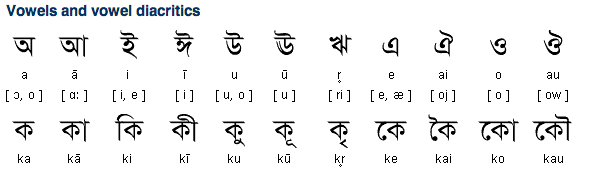
\includegraphics[scale=0.35]{vowels}
  \label{vowels}
\end{figure}
\begin{figure}[h]
  \caption{Consonants in Bengali script.}
  \centering
  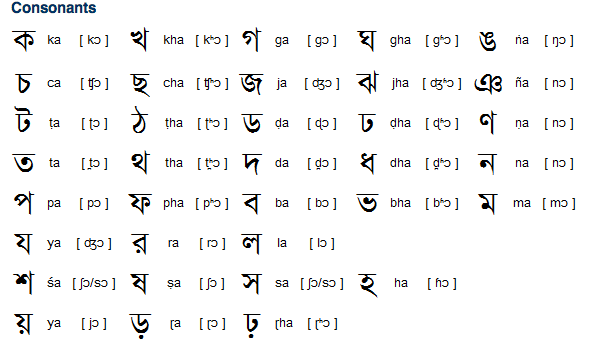
\includegraphics[scale=0.35]{consonants}
  \label{cons}
\end{figure} \\

\section{Past work on Bengali dependency parsing}

Some work has been done in building dependency parsers for Bengali. \citep{ghosh2009dependency} have used a statistical CRF based model followed by a rule based post processing technique. \citep{Nivre_parsingindian}, \citep{ambati_09} used a transition based dependency parsing model based on MaltParser \citep{Nivre05maltparser:a}. \citep{De_Dep_ben} uses a hybrid approach where they simplify the complex and compound sentential structures and then recombine the parses of the simpler structure by satisfying the demands of the verb groups. \citep{bidir_parser} use a bidirectional parser with perceptron learning with rich context as features. \citep{kosaraju_10} used Maltparser and explored the effectiveness of local morphosyntactic features chunk features and automatic semantic information. \citep{attardi_10} used a transition based dependency shift reduce parser which used a Multi layer Perceptron classifier. They were all tested on the same dataset as a part of a shared task held at ICON 2009 and 2010. \citep{husain_09, husain_10}. In the 2009 contest, \citep{ambati_09} system performed the best and in 2010, best score of Unlabeled Attachment Accuracy was achieved by \citep{attardi_10} and the best scores for Label Accuracy and Labeled Attachment was achieved by  \citep{kosaraju_10}.

\section{Existing useful resources for the task}
Microsoft Research India has a POS tagged dataset for several Indian languages including Bengali. The bengali dataset has 899 POS tagged sentences. Also I have been able to gain access to the annotated dataset which was used in the shared task held at ICON 2009 and 2010. Although I am aware that I cannot use the annotated dataset, I am hopeful that it will provide important insights for annotation. The data was annotated using the Computational Paninian Grammar. \citep{Bharati}



\newpage


\bibliographystyle{plainnat}
\bibliography{refs}
\label{lastpage}
\end{document}
